\chapter{Signal Analysis}
\label{Ch:SignalAnalysis} \lhead{Chapter 6. \emph{Signal Analysis}}
The analysis of signals is central to many fields of engineering. In this context, a \textit{signal} is some measurable output of a system. Many operations, such as finding resonant frequencies, can be performed with relative ease in the frequency domain, but are prohibitively expensive in the time domain. Therefore expressions for the signals are often sought in the frequency domain, that to say, as a linear combination of complex sinusoids. Additionally, these complex sinusoids are eigenfunctions of linear, time-invariant systems, such as those described by Maxwells' equations,~\eqref{}. In many real-world applications, time-continuous expressions for these signal are not readily available, and rather the signal values are known only at discrete, uniformly spaces points in time. This chapter will be concerned with the frequency domain representation of continuous, complex-valued time domain signals, which have been discretely sampled.

The term \textit{signal}, or \textit{discrete signal}, is used to refer to $N$ \textit{ samples }, consisting of the values of some continuous complex function at evenly spaced, sequential points in time over a time period $T$. It is convenient to consider this as a vector, in the space the complete, linear vector space $ \{ \ComplexSet^{N} \}$.

The frequency domain representation a signal in the frequency domain will be given by a linear combination of discrete sinusoids. To simply notation, these are represented in complex form, as $ A e^{i (\omega \dtime + \phi) } $, where $A$ is the complex peak amplitude (or equivalently the modulus), $\omega$ is the angular frequency of the oscillation in radians per unit time, $\phi$ is the phase, and $\dtime = n\sampleInterval$ with $n = 0,1,...,N-1$ are the $N$ discrete sample times, at intervals of $\sampleInterval$ in $\sampleInterval$.
% TODO: verify the definition of t_n

Note however that by use of Eulers' identity, any discrete real sinusoid, can be expressed as a linear combination of discrete complex sinusoids with frequencies $\pm \omega$, as
% VIVA: linear combination because cos is also a sinusoid with a different phae
\begin{align*}
A \sin(\omega \dtime + \phi) = \frac{A}{2i} \left( e^{i (\omega \dtime + \phi)} - e^{- i (\omega \dtime + \phi)} \right),
\end{align*}
%It will be seen that the Fourier transform is linear, and therefore results obtained with complex sinusoids are also valid for real sinusoids.
% TODO: Is this the statement I should make ^ - i made up the whole 'linear' thing
Note that any superposition of sinusoids at a given frequency with arbitrary phase and amplitude can always be written as a single sinusoid of the same frequency which has some phase, determined by the phase and amplitude of the summed sinusoids.

% TODO - state somewhere (results) that phase is not so interesting...?
% TODO... justify that signals can be expressed as a series of sinusoids?
% TODO - I've not mentioned anything in an FEM context, or what the Signal is in this context.

\section{The discrete Fourier basis}
The discrete Fourier transform will be introduced as a change of basis in a Hilbert space. By orthogonal projection, the vector signal is written as a weighted linear combination of discrete, complex sinusoids.
% mention something about the coefficients of the linear combination? and how they're the important thing?

First a Euclidian norm is introduced on $\ComplexSet^N$,
$$
\norm{\tdSignal}_{2} \equiv \sqrt{\DFTsum |\tdSignalSample|^2}
,
$$
and by an inner product between any two vectors, $\sigSpaceVectOne$ and $\sigSpaceVectTwo$, in this space as
$$
\left< \sigSpaceVectOne, \sigSpaceVectTwo \right>
\equiv \DFTsum \sigSpaceVectOneComp \complexConj{\sigSpaceVectTwoComp}
$$
% TODO: not defined x_n, u_n, v_n
a Hilbert space is obtained, in which all $N$-sampled signals can be treated as vectors.

The inner product between any two $N$-sampled discrete sinusoids, $\dSinOneNonDFT(\dtime)$ and $\dSinTwoNonDFT(\dtime)$, of arbitrary frequencies $\omegaSinOne$ and $\omegaSinTwo$ respectively is written as
\begin{align}
  \left< \dSinOneNonDFT, \dSinTwoNonDFT \right>
  &\equiv \DFTsum \dSinOneNonDFT(\dtime) \complexConj{\dSinTwoNonDFT(\dtime)} \\
  &= \DFTsum e^{i ( \omegaSinOne - \omegaSinTwo) \nDFT \sampleT } \\
  &= \begin{cases}
    \Nsamples & \textrm{for}\ \omegaSinOne = \omegaSinTwo \\
    \frac{ 1 - e^{i ( \omegaSinOne - \omegaSinTwo) \Nsamples \sampleT} }{ 1 - e^{i ( \omegaSinOne - \omegaSinTwo) \sampleT} } & \textrm{otherwise}
,
    \end{cases}
\label{eq:inner-product-general}
\end{align}

where $\complexConj{\Box}$ denotes the complex conjugate of $\Box$, and the final step is acheived by recalling that any complex geometric sequence $x(z_1) \equiv \sum_{n=0}^{N - 1} z_1^n$, can be written as $x(z_1)
\equiv \frac{1-z_1^N}{1-z_1}$ for any $z_1 \in \{\ \ComplexSet\ |\ z_1 \ne 1
\}$.

It can be easily verified from~\eqref{eq:inner-product-general} that the set of discrete sinusoids which are periodic in $\sampleT$, $\{ e^{i \omegaSinAny \dtime} |\ \omegaSinAny \equiv \frac{2 \pi k  \samplingFreq}{N},  k = 0,1,2,...\Nsamples-1 \}$, which will be referred to as the \textit{discrete Fourier basis}, is an orthogonal set. Following a procedure similar to~\eqref{eq:inner-product-general}, the inner product between two members of this set, $\dSinOne$ and $\dSinTwo$, is given by

$$
\left< \dSinOne, \dSinTwo \right> =
    \begin{cases}
      N, & \text{for}\ \dSinOneIndex = \dSinTwoIndex \\
      0, & \text{for}\ \dSinOneIndex \ne \dSinTwoIndex
    \end{cases}
    ,
$$
with a norm for this set given by
\begin{align*}
  \norm{\dSinOne}
  &= \left< \dSinOne, \dSinOne\right>^{1/2} \\
  &= \sqrt{ \DFTsum e^{i 2 \pi(\dSinOneIndex-\dSinOneIndex) \nDFT / \Nsamples} }
\\ &= \sqrt{N}
,
\end{align*}
The discrete Fourier basis is said to form a basis for $\ComplexSet^{N}$, in which any discrete, $N$-sampled signal may be expressed. Note that this is a finite set, in contrast with the continuous Fourier basis, consisting of $\Nsamples$ discrete sinusoids, at regularly spaces frequencies between $0$ and $\omegaSampling = 2 \pi / \sampleInterval$. The basis could be selected in principle with any arbitrary amplitude and phase, for simplicity however unit amplitude and zero phase complex sinusoids are used.
% TODO - check the sample interval upper limit^^^
% VIVA : the basis is written with the same amplitude and phase (phase is necessary for orthogonality, amplitude for normalisation). Verify this and do the maths.

The \textit{ discrete frequency spectrum }, $\Spectrum(\omegaSinAny)$, of the discrete signal $x(\dtime)$ is defined by convention as $N$ times the coefficient of the projection of the signal onto the $k$th basis function, given by
$$
\Spectrum(\omegaSinAny) = \frac { N \left< x, \dSinAny \right> }{\norm{\dSinAny}^2}
$$
and will be referred to as the \textit{ frequency spectrum } or \textit{frequency domain representation} or simply \textit{spectrum} of $\tdSignal(\dtime)$. This can be thought of as a measure of the amplitude and phase of the $k$th complex sinusoid present in the input signal at frequency $\omegaSinAny$. The spectrum is written explicitly, by substitution, as
\begin{equation}
  \Spectrum(\omegaSinAny)
  \equiv \DFTsum x(\dtime) e^{-i 2 \pi \dSinAnyIndex \nDFT / \Nsamples }\ \ \textrm{for}\ \dSinAnyIndex = 0,1,...,\Nsamples - 1
  \label{eq:dft}
  ,
\end{equation}

An alternative approach is possible, in which an orthonormal set is defined by normalisation of the discrete Fourier basis, and the spectrum is then defined without the factor of $N$, and either approach could be adopted.

The correponding inverse transform, which allows the discrete signal $\tdSignal(\dtime)$ to be recovered from $\Spectrum(\omegaSinAny)$, is simply the sum of projections,
$$
\tdSignal(\dtime) = \sum_{k=0}^{N-1}\frac { \left< x, \dSinAny \right> }{\norm{\dSinAny}^2} \dSinAny
$$
or by substitution
\begin{equation}
  x(\dtime) = \frac{1}{N} \DFTsum \Spectrum(\omegaSinAny) e^{i 2 \pi \dSinAnyIndex \nDFT / \Nsamples }
  \label{eq:idft} ,
\end{equation}
Equations~\eqref{eq:dft} and~\eqref{eq:idft} are known respectively as the discrete Fourier transform (DFT) and the inverse discrete Fourier transform (IDFT) of $\tdSignal(\dtime)$. The process of sampling a continuous signal, to obtain $\tdSignal(\dtime)$, and transforming to its frequency domain representation, $\Spectrum(\omegaSinAny)$, using~\eqref{eq:dft}, is referred to as \textit{Fourier analysis}, or simply \textit{signal analysis}, of $\tdSignal(\dtime)$. The inverse process, whereby an approximate or exact expression of a sampled time domain signal, $\tdSignal(\dtime)$, is obtained from $\Spectrum(\omega_k)$, using~\eqref{eq:idft}, is referred to as Fourier synthesis.

It is interesting to note that computing the Fourier transform of a signal of length $T$ is equivalent to extending that signal periodically with a period $T$. It can be shown easily verified that the discrete Fourier transfrom is a linear operation, since for any $x,y \in \ComplexSet^{N}$ and any $\alpha,\beta \in \ComplexSet$ the DFT satisfies
$$
\alpha x + \beta y \to \alpha X + \beta Y
$$
as is readily demonstrated by substitution:
\begin{align*}
  DFT_k [ \alpha x + \beta y]
  &\equiv \sum_{n=0}^{N-1} \left[ \alpha x(n) + \beta y(n) \right] e^{-j 2 \pi n k / N} \\
  &= \alpha \sum_{n=0}^{N-1} \alpha x(n) e ^ {-i 2 \pi n k /N} + \beta \sum_{n=0}^{N-1} y(n) e^{-i 2 \pi n k / N} \\
  &\equiv \alpha DFT_k[ x ] + \beta DFT_k[ y ]
\end{align*}
where $X$ and $Y$ are respectively the discrete fourier transforms of $x$ and $y$, and $DFT_k[\Box]$ indicates the $k$th component of the DFT transform of $\Box$.
%** also the maxwells equations are linear....so what...?

\section{Aliasing}
Let $\downSampleSpectrum$ be the spectrum of the downsampled signal $\downSampleSignal(L \dtime)$ of length $M$, obtained by downsampling $\tdSignal(\dtime)$, that is the vector of every $L$th sample of $\tdSignal$, with $ M = N/L$. $\downSampleSpectrum$ can be written in the form
\begin{align}
Y(k') = \sum_{m=0}^{M-1} x(mL) e^{- i 2 \pi k' m / M} \frac{1}{L} \sum_{l=0}^{L-1} \left(  e^{-i 2 \pi n / L} \right)^l \label{eq:sig:downsampled-signal}
\end{align}
where the sum over $l$, using the closed form geometric series in~\eqref{}, is non-zero only for integer multiples of $L$ samples,
\begin{align*}
\frac{1}{L} \sum_{l=0}^{L-1} \left(  e^{-i 2 \pi n / L} \right)^l =  \frac{ 1 - e^{- i 2 \pi n }}{ L (1 - e ^{-i 2 \pi n/ L})} =
  \begin{cases}
   1, & n = 0,L,2L,3L,...,(M-1)L  \\
   0, & \textrm{otherwise}
  \end{cases}
        .
\end{align*}
This expression is equivalent to the discrete Fourier transform of $\downSampleSignal(L \dtime)$, with only a change of index of the summation, and the addition of zero summation terms. Equation~\eqref{eq:sig:downsampled-signal} can be rewritten, by simple algebraic manipulations, as
\begin{align*}
Y(k')
  %&= \sum_{n=0}^{N-1} x(n) e^{-i 2 \pi k' n / N} \sum_{l=0}^{L-1} \left(  e^{-i 2 \pi n / L} \right)^l \\ 
  %&= \sum_{n=0}^{N-1} x(n) e^{-i 2 \pi k' n / N} \sum_{l=0}^{L-1} e^{-i 2 \pi lM n / N} \\
  &= \frac{1}{L} \sum_{l=0}^{L-1} \sum_{n=0}^{N-1} x(n) e^{-i 2 \pi (k' + lM) n / N} \\
  &= \frac{1}{L} \sum_{l=0}^{L-1} X(k' + lM) .
\end{align*}
Thus downsampling of $\tdSignal(\dtime)$ by a factor $L$ results in a spectrum of length $M = N / L$, equivalent to dividing the spectrum $X$ into $L$ continuous ranges by index, and summing the corresponding indicies in each range, as illustrated in figure~\ref{fig:illustration-of-spectral-ranges}.

Spectral components above $k'$ in the original spectrum are said to be \textit{folded} or \textit{mirrored} into the spectrum. Frequency components at $\freqSample + \freqSampleAbove$, where $\freqSample \equiv 1/\sampleInterval$ is the sampling frequency, will contribute to a peak in the resulting frequency spectrum at the frequency $\freqSample - \freqSampleAbove$, for $\freqSampleAbove \le \freqSample / 2$, and is said to alias to a lower frequency. This loss of information is not reversible in general. The two frequencies cannot be distinguished in the resulting spectrum, and the original signal can no longer be reconstructed exactly from its spectrum.
% equiv to changing the radius of the unit circle in the $z$-plane along which the discrete Fourier basis function set is selected.

If $X(k')$ is bandlimited in the frequency domain such that it is zero for any $k' + lM > M$, then $Y(k') = X(k')$, and the downsampling of the signal results in no loss of information.

The well known sampling theorem, first proposed by Harold Niquist in 1928 and
later revived by Claude Shannon, states that any continuous, bandlimited signal, $\tdSignal(t)$, can be reconstructed exactly from its samples by sinc interpolation,
$$
\tdSignal(t) \equiv \sum_{n=0}^{N-1} x(\dtime) \
\textrm{sinc}\left( \freqSample (t-t_{n}) \right),
$$
provided there is no energy in the signal frequency spectrum at or above half
the sampling frequency. This upper frequency limit is referred to as the
\textit{Niquist frequency}, $\NiquistFreq$, and the corrisponding minimum sampling rate is referred to as the \textit{Niquist rate}.

In practice aliasing effects can also be reduced by applying a low-pass filter to the signal to remove all energy at a frequency of $\freqSample / 2$ and above. Perfect low-pass filters, which remove completely only frequencies above a given cut-off frequency, without modifying frequencies below, are only possible for infinitely long signals. However, low-pass filters with sufficiently narrow transition regions can usually be realised.

In a finite element context, it is convenient to write the Niquist frequency as a lower limit on simulation time step
$$
\NiquistFreq < \frac{1}{2 \Delta t} .
$$
%NOTE: Should I introduce the concept of thinking of FEM as a low pass filter??? Solves aliasing problems.

% represented fully...

\section{Spectral Leakage}
% TODO: talk about periodic extension here.... 
If the function from which $\tdSignal$ is sampled has a periodicity which is an integer divisor of $T$, and can therefore be expressed as a linear superposition of continuous sinusoids of the frequencies of the discrete Fourier basis, then original continuous function can be synthesised exactly given the values of $\Spectrum(\omegaSinOne)$.

For signal obtained from source which contains frequencies different from the basis frequency, this is not the case. Whilst the synthesised function and the original sampled function will be exactly identical at the $N$ sample points, the intermediate, interpolated values may differ.
% TODO: IS THIS TRUE....!??? Isnt this the point of the DFT for this NOT to be the case? Should I verify this.
Further insight can be obtained by looking at the contribution of a sinusoid at frequency $\omegaContrib$ to the $\dSinAnyIndex$th fourier basis function, by computing its orthogonal projection onto $\dSinAny$, as
%% TODO : NEED TO SHOW THAT ANYTHING IS EXPRESSABLE AS A SIN WAVE _ OTHERWISE THIS HAS NO MEANING
%%%%%%%%%% TODO : THIS IS ALL CARP...!?? The projection is for sin -> sin....!???
\begin{align*}
  \Spectrum(\omega_k) &= \frac{ 1 - e^{i (\omega_f -
\omega_k) N T} }{1 - e^{i(\omega_f - \omega_k) T}} \\ &= \frac{ \sin[(\omega_f -
\omega_k)N T / 2]}{\sin[(\omega_f - \omega_k) T / 2]} e^{i (\omega_f - \omega_k)
(N - 1) T /2} .
\end{align*}
This absolute value of this expression, is plotted against $\omegaContrib$ in~\ref{fig:amplitude-contribution-to-component-by-freq}, is interpreted as the amount which any frequency, $\omegaContrib$, contributes to $\Spectrum(\omegaSinAny)$. The largest contribution to $\Spectrum(\omegaSinAny)$ comes from the frequency $\omegaSinAny$, as exepected. Since the discrete Fourier basis function are mutually orthogonal, the contribution from the other discrete Fourier frequencies is zero. The largest frequency contribution is given by sinusoids in the frequency bin $\omega_{k - 1/2}$ and $\omega_{k+1/2}$, known as the \textit{main lobe}, however contributions are also made by sinusoids in all frequency bins.
\begin{figure}[h] \centering
  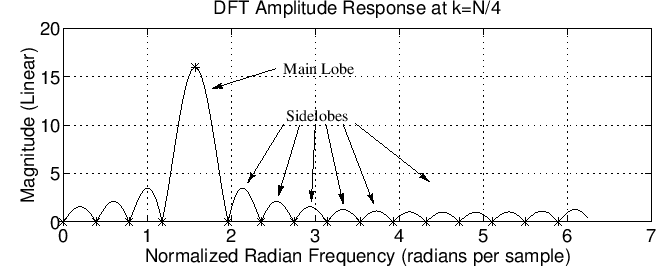
\includegraphics[width=\textwidth]{Figures/Chapters/SignalAnalysis/spectralLeakage}
  \caption{Plot showing the amplitude contribution of a sinusoid at any frequency $\omega_f$ to a given spectral component}
  \label{fig:amplitude-contribution-to-component-by-freq}
\end{figure}
This phenomena is known as \textit{spectral leackage} and is due to
discontinuites caused by periodic extension of functions which do not exhibit
periodicity $T$. Spectral leakage is exhibited at all frequencies
except for the discrete Fourier basis frequencies, which are the only sinusoids
which are continuous under periodic extension. Note that peak leakage is not reduced by increasing $N$\cite{}.
% TODO - more on input signal being the same as its extension -> Section 7.1.2

\section{Window Functions}
Choosing a sample length, $sampleT$, for which all sinusoidal frequency
components are periodic is rarely possible or desirable in practical
applications. Whilst spectral leakage cannot be eliminated, the contribution
made to a component by distant frequency can be reduced by an appropriate choice
of window function. In this context, the process of sampling a signal over a
finite length of time is equivalent to multiplication by a rectangular window,
such as the one shown in~\ref{fig:rectangular-window}, or equivalently convolution with the Fourier transform of the window, shown in~\ref{fig:rectangular-window-FT}, in the frequency domain.
Truncation of the signal at the window endpoints gives rise to spectral leakage.
Window functions which gradually tapers to zero at the endpoints of the sample
interval are often used, resulting in a continuous periodic extension. This has
the effect of widening the main lobe and reducing the amplitude of the side
lobes compared to the leakage of a rectangualar wave shown
in~\ref{fig:amplitude-contribution-to-component-by-freq}.

The choice of window function should depend on the dynamic range of the input signal and the required resolution. Several popular choices of window functions and their spectra are shown in~\ref{fig:popular-window-functions}. Several choices of window functions are considered, including the Blackman window\cite{} given by
% REF: Blackman, R. B. and Tukey, J. W. "Particular Pairs of Windows." In The Measurement of Power Spectra, From the Point of View of Communications Engineering. New York: Dover, pp. 98-99, 1959.
$$
W(x) = \frac{21}{50} \frac{1}{2} cos ( \frac{\pi x}{a} ) + \frac{2}{25} cos (
\frac{2 \pi x }{a} )
$$
and the Hamming window\cite{}, given by
$$
W(x) = \alpha - \beta \cos\left(\frac{2 \pi n}{N - 1}\right)
$$
with $\alpha = 0.53836$ and $\beta = 0.46164$, and the Blackman-Nutall window\cite{}, given by
$$
W(x) = a_0 - a_1 \cos \left( \frac{ 2 \pi n }{N - 1} \right) + a_2 \cos \left(
  \frac{ 4 \pi n }{ N - 1} \right) - a_3 \cos \left( \frac{ 6 \pi n }{N - 1} \right)
$$
with $a_0 = 0.35875$, $a_1 = 0.48829$, $a_2 = 0.14128$ and $a_3 = 0.01168$.
\begin{figure}[h] \centering
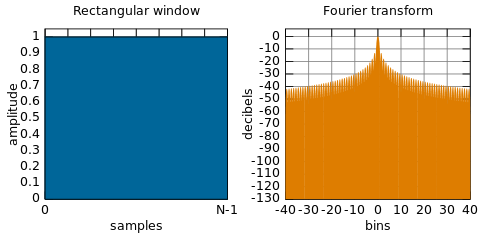
\includegraphics[width=0.5 \textwidth]{Figures/Chapters/SignalAnalysis/Windows/rectangularWindow}
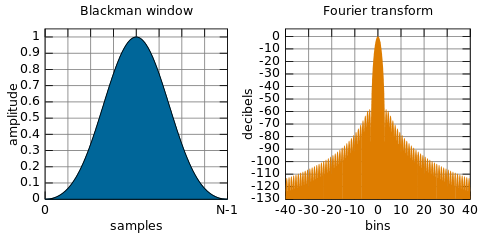
\includegraphics[width=0.5 \textwidth]{Figures/Chapters/SignalAnalysis/Windows/BlackmanWindow}
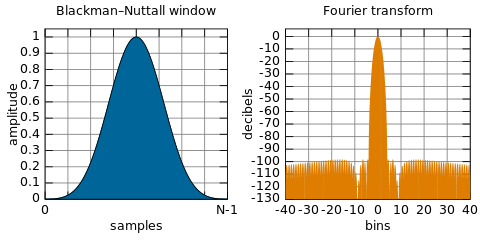
\includegraphics[width=0.5 \textwidth]{Figures/Chapters/SignalAnalysis/Windows/BlackmanNutallWindow}
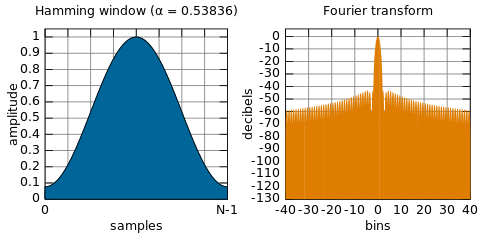
\includegraphics[width=0.5 \textwidth]{Figures/Chapters/SignalAnalysis/Windows/HammingWindow}
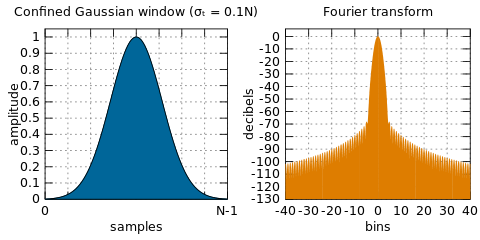
\includegraphics[width=0.5 \textwidth]{Figures/Chapters/SignalAnalysis/Windows/ConfinedGaussianWindow}
  \caption{Plot showing the amplitude contribution of a sinusoid at any frequency $\omega_f$ to a given spectral component}
  \label{fig:amplitude-contribution-to-component-by-freq}
\end{figure}
% TODO - some statement about not reducing peak leakage...but rather a tradeoff between resolution and dynamic range...
% TODO - something about Rect window making peaks hard to find, but having high resolution.
\subsection{Symmetry}
For real input signals where $x \in \Real^N$, its spectrum exhibits symmetry
about zero. This is verified by writing the flipped spectrum,
\begin{align*}
  \Spectrum(-k)
  &\equiv - \sampleT x(n) \DFTexp{( -k )} \\
  &= \overline{ \DFTsum \overline{x(n)} \DFTexp{k}} \\
  &= \overline{ \DFTsum x(m) \DFTexp{k}} \\
  &= \overline{\Spectrum(k)}
\end{align*}
For a real signal, $\RealPart{\Spectrum(k)}$ and $|\Spectrum(k)|$ are even symmetric functions and $\ImagPart{\Spectrum(k)}$ and $\angle \Spectrum(k)$ are odd symmetric functions. Due to this symmetry, only positive frequencies (from $0$ and $\samplingFreq/2$) are plotted when presenting spectra, since negative frequencies contain no additional information.
% TODO - be more specific about what is meant by FLIP(x) or x(-n)...
% note, I haven't proved that the angle or magnitude are even/odd here...but it follows from conjugate summetry of X in polar form $X(k) = |X(k)|e^{i \angle X(K)}$ i.e. just write X(k) in polar form and its immediately obvious...is it?

%%%%  TIME REVERSAL
%\begin{align*}
%  DFT_k(-x)
%  &\equiv \DFTsum x(N-n) \DFTexp{k} \\
%  &= \sum_{m=0}^{N-1} x(m) e^{- i 2 \pi (N-m)k / N} \\
%  &= \sum_{m=0}^{N-1} x(m) e^{- i 2 \pi m ( -k ) / N} \\
%  &\equiv \Spectrum(-k)
%\end{align*}
%Therefore for any real signal reversal of the signal in time leads to reversal of the spectrum.

%%%%  Zero phase signals
% \begin{quote} Definition: A signal with a real spectrum (such as any real, even signal) is often called a zero phase signal. However, note that when the spectrum goes negative (which it can), the phase is really $ \pm\pi$ , not 0 . When a real spectrum is positive at dc (i.e., $ X(0)>0$ ), it is then truly zero-phase over at least some band containing dc (up to the first zero-crossing in frequency). When the phase switches between 0 and $ \pi $ at the zero-crossings of the (real) spectrum, the spectrum oscillates between being zero phase and ``constant phase''. We can say that all real spectra are piecewise constant-phase spectra, where the two constant values are 0 and $ \pi $ (or $ -\pi$ , which is the same phase as $ +\pi$ ). In practice, such zero-crossings typically occur at low magnitude, such as in the ``side-lobes'' of the DTFT of a ``zero-centered symmetric window'' used for spectrum analysis (see Chapter 8 and Book IV [73]). \end{quote}

\section{Zero Padding \& Interpolation}
In order to obtain high spectral resolution, a small $\deltaFreq$ is desirable.
Often sampling the input signal over a sufficiently long $T$ to obtain the desired resolution is impractical. In such cases interpolation methods are often used. It can be shown that zeros padding a causal signal (that is a signal which is zero before $t=0$), corresponds to \textit{ideal bandlimited interpolation} in the frequency domain. Let $\zeroPadSignal(\dtimeZeroPad) \in \ComplexSet^{M}$ be a signal of length $M$, obtained by zero padding a signal $\tdSignal \in
\ComplexSet^{N}$ with zeros, such that
\begin{align*}
  \zeroPadSignal(\dtimeZeroPad) =
  \begin{cases}
    \tdSignal(\dtimeZeroPad) & \textrm{for}\ \dtimeZeroPadIndex \in [0,N-1] \\
    0 & \textrm{for}\ \dtimeZeroPadIndex \ge N
  \end{cases}
\end{align*}
The DFT of $\zeroPadSignal(\dtimeZeroPad)$ is given by
\begin{align*}
  DFT_k(\zeroPadSignal)
  &= \sum_{m=0}^{M-1} \zeroPadSignal(m) e^{- i 2 \pi m k' / N} \\
  &= \sum_{n=0}^{N-1} \zeroPadSignal(n) e^{- i 2 \pi n k' / N} \\ &= \Spectrum(\omega_{k'})
,
\end{align*}
where $\Spectrum(\omega_{k'})$ is the coefficient of projection of $x(n)$ onto a discrete Fourier transform sinusoid of frequency $\omega_{k'}$. Such interpolation is exact for a time-limited signal, which is truly zero outside of the window. Zero padding will not however improve spectral resolution, or increase the amount of information contained in the spectrum. Zero padding is generally performed after applying a suitable window function.
% VIVA / TODO :what about non-time-limited???? Apparently this differs....? I
% think in this case I just get spectral leakage

Since the FFT algorithm allows rapid computation of the DFT, padding the time
domain signals with zeros prior to and FFT is often an efficient and accurate
interpolation method.
% QIFFT method:
% https://www.dsprelated.com/freebooks/sasp/Sinusoidal_Peak_Interpolation.html

% J. O. Smith and X. Serra, ``PARSHL: A program for the analysis/synthesis of inharmonic sounds based on a sinusoidal representation,'' in Proceedings of the 1987 International Computer Music Conference, Champaign-Urbana, Computer Music Association, searchable at http://quod.lib.umich.edu/i/icmc/, 1987, 

% M. Abe and J. O. Smith, ``Design criteria for simple sinusoidal parameter estimation based on quadratic interpolation of FFT magnitude peaks,'' Audio Engineering Society Convention, San Francisco, 2004, 

%review paper (I think) https://ai2-s2-pdfs.s3.amazonaws.com/7bbc/c4d13458d0a6570fba35f508c2b44444fb07.pdf
The location of spectral peaks may be obtained by so-called quadratically
intepolated FFT(QIFFT). This consists of finding the location of the peak as the
maxima of the parabola formed by the three points of the spectrum of a zero
padded signal nearest the peak. The QIFFT method may be considered an approximate maximum likelihood method for spectral peak estimation. This approach is valid for any window, since for points in a region sufficiently close to a peak, the higher order terms in a Taylor series expansion about the peak converge to zero as the peak is approached. This is often more computationally efficient than zero padding alone.

In the case of the Gaussian window however, since the window transform is
exactly a parabola on a log scale, the parabolic approximation in exact for
infinite windows. In practice however, small error may be introduced due to truncation.
% show an example of the Gaussian window....?
Neither choice of interpolation method improves the resolution of the spectrum, which is related to the window shape and length.
% VIVA: related to amount of information
% VIVA: what does this mean
% what is ``upsampling'' - alternative approach?
\section{Quality Factor}
The quality factor is a widely used in engineering to describe the damping of an
oscillating system. The qaulity factor, $Q$, indicates the rate at which energy
is dissipated in the system. In applications where resonance is required,
engineering a system with a high-Q is usually desirable. In a high-Q system
resonant frequency oscillations will have a longer lifetime and less energy need
be provided to the system to maintain an oscillation. The Q-factor at a resonant
frequency, $f_{res}$ commonly written as the ratio

$$
Q = f_{res}/\B_{FWHM}
$$

where $B_{FWHM}$ is the bandwith of the resonant oscillation at half of its
amplitude, commonly known as the full-width-half-maximum (FWHM) value. An
equivalent definition can be given in terms of the ratio of energy stored in the
oscillator at resonant frequency to the rate of energy loss per cycle

In a resonant optical cavity the quality factor, $Q$, for a given resonant
frequency, $f_{res}$, is given by

$$
Q = 2 \pi f_{res} \frac{\Epsilon}{P}
$$

where $\Epsilon$ is the energy stored in the system and $P$, the dissipated
power, is given by $-\frac{d \Epsilon}{dt}$.

In resonant system with a high quality factor, resonant frequency oscillations
with have a long lifetime. Whilst oscillations away from the resonant frequency
will die out quickly. Conversely in a system with a lower Q-factor the resonant
oscillations will die out quickly and the resonant peak will have a larger
bandwidth. 

For a dispersive system this will manifest itself in a broadening spectrum line width [], and consequentially a larger error in the quality factor. Note that
dispersion could be either physical or could be a non-physical dispersion
introduced by a numerical method.

%WWWIIK

% *** maybe mention Q-switching - how does Q-switching work? Am I going to research it?

\section{Lorentzian line shapes}
FWHM -> decay time. Conversion between FWHM and decay time
http://physik.uni-graz.at/~atr/publications/phd-thesis.pdf [p.189]

% about absorbtion mode: http://www-keeler.ch.cam.ac.uk/lectures/understanding/chapter_4.pdf

\section{FFT}
* present FFT as a way of computing DFT * who came up with it *
how important is it
* how much faster is it
* we don't have anything faster for a GENERAL signal
* none of this would be possible (i.e. DFT is too slow) without FFT

The widely used Fast Fourier transform [***] algorith which reduces the computational of the DFT from an $\bigO(n^2)$ operation to an $\bigO(n log n)$ operation. 

\section{Alternatives} * These work for SPECIFIC cases.... STFT (short time fast
fourier transform) -> at least get a reference and some comments with reference to existing work 
%http://repository.cmu.edu/cgi/viewcontent.cgi?article=1065&context=dissertations
z-transform - smaller windows spare FT - zero outputs (not intersting I don't think)
FDM - constrained to decaying outputs (solve eigenvalue problem)
%methods (supposedly) designed to reduce truncation * maxiumum entropy * linear prediction * FDM
% thats what it says in
%http://www-keeler.ch.cam.ac.uk/lectures/understanding/chapter_4.pdf




http://researchrepository.napier.ac.uk/4022/1/phd.pdf [p.43] <- some references
here parametric approaches - what are these? non-parametric approaches - what
are these?

MY BUMPH...
Parametric methods such as the filter diagonalisation method (FDM) use an
assumption of the shape of the signal to find the resonant frequencies by
solving an eigenvalue problem. This method can be used to significantly reduce
the error in the number time steps required to reach a solution. In numerical
experiements a increase of an order of mangnitude was observed for FDM over FFT.

However parametric methods are sensitive to dispersion which can degrade the
signal amplitude for signals which are of a considerable length, and therefore
while a better result can be obtained for a short run, for longer runs required
to obtain a high accuracy the method is unsuitable.
\section{TODO}
The spacing of the discrete points in frequency space, is given by
$$
\Delta f = \frac{1}{T}
$$
where $T$ is the final time of the simulation. Care should be taken to ensure
that the final time of the simulation is sufficiently long to account for the
desired simulation error.

DFT does not require integrals over infinite limits to be calculated (i.e. calculus), as in FT
% https://ccrma.stanford.edu/~jos/st/Introduction_DFT.html

nice page on definitions
%https://ccrma.stanford.edu/~jos/mdft/DFT_Definition.html

* example of what a spectrum looks like * what are the peaks, what is resonance
etc * Quantities of interest * Peak height * Peak width (Quality factor
calculations) * FSR * phase

* mention zero frequencies

* LTI and Maxwells equations being an LTI system...? Sinusoids are eigenvalues of LTI systems.

* Parsevals Theorem

RESULTS: A system with PEC boundaries and no material loss with no numerical errors is expected to have a zero linewidth and infinite quality factor.

QUESTION: also discuss RESONANCE in the physical problem section?
mention broad frequency band responses as an advantage of time domain somewhere

MODE SHAPES (GOES IN RESULTS)
The fourier transform can be thought of as a factorisation of the signal into a
temporal and spatial part. For a single point the spatial part will simply be a
complex amplitude. However when the entire domain is considered each point has
an associated complex amplitude for each frequency, which forms a spatial
envelope which when multipled by the temporal part defines the oscillations
associated with that frequency. When the frequency considered is a resonant
frequency, then the envelope is known as the mode shape associated with that
frequency.

% what do I have
** what I have: a discrete-time signal - discrete in x,
* Q: how can we turn the signal which depends on time -> function that depends on frequency (spectrum)

** continuous in y
** finite length
** discretely sampled
** time domain (function of time)

** how this connects with resonance

** what is a signal...?

%%% Local Variables:
%%% mode: latex
%%% TeX-master: "../Thesis"
%%% End:
